\documentclass{article}

\usepackage{arxiv}

\usepackage[utf8]{inputenc} % allow utf-8 input
\usepackage[T1]{fontenc}    % use 8-bit T1 fonts
\usepackage{lmodern}        % https://github.com/rstudio/rticles/issues/343
\usepackage{hyperref}       % hyperlinks
\usepackage{url}            % simple URL typesetting
\usepackage{booktabs}       % professional-quality tables
\usepackage{amsfonts}       % blackboard math symbols
\usepackage{nicefrac}       % compact symbols for 1/2, etc.
\usepackage{microtype}      % microtypography
\usepackage{lipsum}
\usepackage{graphicx}

\title{Vaccinating Australia: How long will it take?}

\author{
    Mark Hanly
   \\
    Centre for Big Data Research in Health \\
    UNSW Sydney \\
  Sydney 2052 \\
  \texttt{\href{mailto:m.hanly@unsw.edu.au}{\nolinkurl{m.hanly@unsw.edu.au}}} \\
   \And
    Tim Churches
   \\
    Ingham Institute for Applied Medical Research \\
    South Western Sydney Clinical School, Faculty of Medicine, UNSW Sydney \\
  Liverpool \\
  \texttt{\href{mailto:timothy.churches@unsw.edu.au}{\nolinkurl{timothy.churches@unsw.edu.au}}} \\
   \And
    Oisín Fitzgerald
   \\
    Centre for Big Data Research in Health \\
    UNSW Sydney \\
  Sydney 2052 \\
  \texttt{\href{mailto:o.fitzgerald@unsw.edu.au}{\nolinkurl{o.fitzgerald@unsw.edu.au}}} \\
   \And
    Louisa Jorm
   \\
    Centre for Big Data Research in Health \\
    UNSW Sydney \\
  Sydney 2052 \\
  \texttt{\href{mailto:l.jorm@unsw.edu.au}{\nolinkurl{l.jorm@unsw.edu.au}}} \\
  }


% Pandoc citation processing

\usepackage{booktabs}
\usepackage{longtable}
\usepackage{array}
\usepackage{multirow}
\usepackage{wrapfig}
\usepackage{float}
\usepackage{colortbl}
\usepackage{pdflscape}
\usepackage{tabu}
\usepackage{threeparttable}
\usepackage{threeparttablex}
\usepackage[normalem]{ulem}
\usepackage{makecell}
\usepackage{xcolor}


\begin{document}
\maketitle

\def\tightlist{}


\begin{abstract}
Enter the text of your abstract here.
\end{abstract}

\keywords{
    COVID19
   \and
    vaccination
  }

\hypertarget{introduction}{%
\section{Introduction}\label{introduction}}

The COVID-19 pandemic continues to wreck devastating health impacts,
having reached 100 million cases and 2.1 million deaths worldwide, as of
1 February 2021. The worsening crisis has led to the hospitals and ICU
departments being overwhelmed in many countries. Australia has escaped
the worst of these health impacts, through a combination of border
closures, local and state-wide lock down measures and effective tracking
and quarantining of exposed individuals. While effective in mitigating
the spread of the virus, these measures have come at a massive cost for
many industries, including tourism, aviation, retail, tertiary education
and the arts. While the program of hotel quarantine has been largely
effective in blocking transmission from international arrivals it is
clearly not a panacea. Sporadic seeding events have spawned community
clusters leading to further disruptive lockdowns in Victoria, Adelaide,
Sydney and Brisbane.

Several COVID-19 vaccines with promising clinical trial results have
been developed or are close to completion, with national rollouts
already begun in many countries including Israel, the United States and
the United Kingdom. The Australian government has entered into four
agreements for the supply of COVID-19 vaccines (Table
\ref{tab:agreements}), with a view to starting vaccination in February.
The national rollout strategy divides the population into 16 groups,
organised into five phases (Table \ref{tab:phases}).\\

\begin{table}[H]

\begin{threeparttable}
\caption{\label{tab:agreements}Australia’s vaccine agreements}
\centering
\begin{tabular}[t]{>{\raggedright\arraybackslash}p{3cm}>{\raggedright\arraybackslash}p{3cm}>{\centering\arraybackslash}p{1cm}>{\raggedright\arraybackslash}p{2cm}>{\raggedright\arraybackslash}p{5cm}}
\toprule
Name & Type & Doses (millions) & Schedule & Status\\
\midrule
\cellcolor{gray!6}{Pfizer/BioNTech} & \cellcolor{gray!6}{mRNA vaccine} & \cellcolor{gray!6}{10} & \cellcolor{gray!6}{2 doses 21 days apart} & \cellcolor{gray!6}{Provisionally approved by the TGA}\\
University of Oxford AstraZeneca & Viral vector vaccine & 54 & 2 doses 28 days apart & Phase 3 clinical trials\\
\cellcolor{gray!6}{Novavax} & \cellcolor{gray!6}{Protein vaccine} & \cellcolor{gray!6}{51} & \cellcolor{gray!6}{2 doses 21 days apart} & \cellcolor{gray!6}{Phase 3 clinical trials}\\
COVAX Facility & Assorted & 25 & Assorted & 9 candidate vaccines in various clinical trial stages\\
\bottomrule
\end{tabular}
\begin{tablenotes}
\small
\item [] Adapted from https://www.health.gov.au/initiatives-and-programs/covid-19-vaccines/about-covid-19-vaccines/australias-vaccine-agreements
\end{tablenotes}
\end{threeparttable}
\end{table}

Hospital hubs with access cold chain storage facilities will administer
the Pfizer/BioNTech vaccine to the highest priority groups scheduled in
Phase 1a, which includes border workers, frontline healthcare staff, and
aged care staff and residents. The prime minister has set an optimistic
target of 80,000 vaccines per day.\textsuperscript{1}

\begin{itemize}
\tightlist
\item
  A back of the envelope calculation would suggest it would take 500
  days to vaccinate 20 million adult Australians twice.
\item
  But there are some complications e.g.~timing of second doses and
  vaccine hesitancy; we are going to need a bigger envelope.
\item
  Aim of this analysis is to calculate how long it will take the
  vaccinate the whole Australian population
\end{itemize}

\begin{table}[H]

\begin{threeparttable}
\caption{\label{tab:phases}Australia’s COVID-19 vaccine national roll-out strategy}
\centering
\begin{tabular}[t]{>{\raggedright\arraybackslash}p{1cm}>{\raggedright\arraybackslash}p{11cm}>{\raggedleft\arraybackslash}p{2cm}}
\toprule
Phase & Description & Size\\
\midrule
\textbf{\cellcolor{gray!6}{1a}} & \cellcolor{gray!6}{Quarantine \& border workers} & \cellcolor{gray!6}{70,000}\\
\textbf{1a} & Frontline health care workers & 100,000\\
\textbf{\cellcolor{gray!6}{1a}} & \cellcolor{gray!6}{Aged care and disability care staff} & \cellcolor{gray!6}{318,000}\\
\textbf{1a} & Aged care and disability care residents & 190,000\\
\textbf{\cellcolor{gray!6}{1b}} & \cellcolor{gray!6}{Elderly adults aged 80 years and over} & \cellcolor{gray!6}{1,045,000}\\
\textbf{1b} & Elderly adults aged 70-79 years & 1,858,000\\
\textbf{\cellcolor{gray!6}{1b}} & \cellcolor{gray!6}{Other health care workers} & \cellcolor{gray!6}{953,000}\\
\textbf{1b} & Aboriginal and Torres Strait Islander people aged 55 years and over & 87,000\\
\textbf{\cellcolor{gray!6}{1b}} & \cellcolor{gray!6}{Younger adults with an underlying medical condition} & \cellcolor{gray!6}{2,000,000}\\
\textbf{1b} & Critical and high risk workers & 196,000\\
\textbf{\cellcolor{gray!6}{2a}} & \cellcolor{gray!6}{Adults aged 60-69} & \cellcolor{gray!6}{2,650,000}\\
\textbf{2a} & Adults aged 50-59 & 3,080,000\\
\textbf{\cellcolor{gray!6}{2a}} & \cellcolor{gray!6}{Aboriginal and Torres Strait Islander people aged 18-54} & \cellcolor{gray!6}{387,000}\\
\textbf{2a} & Other critical and high risk workers & 453,000\\
\textbf{\cellcolor{gray!6}{2b}} & \cellcolor{gray!6}{Balance of adult population} & \cellcolor{gray!6}{6,643,000}\\
\textbf{3} & <18 if recommended & 5,670,000\\
\bottomrule
\end{tabular}
\begin{tablenotes}
\small
\item [] Adapted from https://www.health.gov.au/sites/default/files/documents/2021/01/australia-s-covid-19-vaccine-national-roll-out-strategy.pdf
\end{tablenotes}
\end{threeparttable}
\end{table}

\hypertarget{methods}{%
\section{Methods}\label{methods}}

\hypertarget{population-and-priority-groups}{%
\subsection{Population and priority
groups}\label{population-and-priority-groups}}

Our analysis was based on the 16 priority groups and five phases
proposed by the Australian government (see Table \ref{tab:phases}). This
resulted in an estimated population size of 25.7 million people,
including 5.67 million under the age of 18. Equal priority was given to
all groups within the same phase.

\hypertarget{roll-out-projections}{%
\subsection{Roll out projections}\label{roll-out-projections}}

Roll out projections were based on four parameters:

\begin{enumerate}
\def\labelenumi{\arabic{enumi}.}
\tightlist
\item
  The number of daily available vaccine units \(units_i\)
\item
  The minimum time between the first dose and the second dose.
\item
  The maximum time between the first dose and the second dose.
\item
  Vaccine hesitancy
\end{enumerate}

\hypertarget{vaccine-allocation}{%
\subsection{Vaccine allocation}\label{vaccine-allocation}}

We allocated the daily available vaccination doses according to the
following broad steps:

\begin{enumerate}
\def\labelenumi{\arabic{enumi}.}
\item
\end{enumerate}

\hypertarget{projection-scenarios}{%
\subsection{Projection scenarios}\label{projection-scenarios}}

\begin{itemize}
\tightlist
\item
  Vary three factors with two levels each resulting in 8 scenarios (see
  Table 2)
\item
  Daily vaccination capacity (60,000 versus 80,000)
\item
  Timing between first and second dose (3 to 6 weeks, versus 3 to 12
  weeks)
\item
  Vaccine hesitancy (7\% versus 13\%) based on recent survey data from
  Edwards et al (the projections assume taht hesitancy applies to
  general population groups but not to health or border workers, age
  care residents or those with an underlying condition)
\item
  Assume that the vaccine is administered according to the priority
  phases set out by the government
\item
  All groups within a given phase are given equal priority
\item
  Daily capacity is first divided between those needing second dose to
  ensure all second doses are delivered within the specified window; the
  remainder of the daily capacity distributed among those requiring
  their first dose.
\end{itemize}

The analysis was performed using RStudio version 4.0.3. The source code
can be accessed at \url{https://github.com/CBDRH/vaccinatingAustralia}.

\begin{table}[H]

\caption{\label{tab:scenarios}Projection scenarios}
\centering
\begin{tabu} to \linewidth {>{}l>{\raggedleft}X>{\raggedleft}X>{\raggedleft}X}
\toprule
Scenario & Capacity (units per day) & Gap between doses & Hesitancy\\
\midrule
\textbf{\cellcolor{gray!6}{1}} & \cellcolor{gray!6}{80,000} & \cellcolor{gray!6}{3 to 6 weeks} & \cellcolor{gray!6}{7\%}\\
\textbf{2} & 80,000 & 3 to 6 weeks & 13\%\\
\textbf{\cellcolor{gray!6}{3}} & \cellcolor{gray!6}{80,000} & \cellcolor{gray!6}{3 to 12 weeks} & \cellcolor{gray!6}{7\%}\\
\textbf{4} & 80,000 & 3 to 12 weeks & 13\%\\
\textbf{\cellcolor{gray!6}{5}} & \cellcolor{gray!6}{60,000} & \cellcolor{gray!6}{3 to 6 weeks} & \cellcolor{gray!6}{7\%}\\
\textbf{6} & 60,000 & 3 to 6 weeks & 13\%\\
\textbf{\cellcolor{gray!6}{7}} & \cellcolor{gray!6}{60,000} & \cellcolor{gray!6}{3 to 12 weeks} & \cellcolor{gray!6}{7\%}\\
\textbf{8} & 60,000 & 3 to 12 weeks & 13\%\\
\bottomrule
\end{tabu}
\end{table}

\hypertarget{results}{%
\section{Results}\label{results}}

\begin{itemize}
\item
  Under the most optimistic Scenario (Scenario 1), assuming vaccination
  starts on March 1, the highest priority group would be fully
  vaccinated with two doses by April 16th, just over six weeks (see
  Table 4).
\item
  However it would still take nearly nine months to complete Phase 2a,
  which includes adults aged 60-69 years.
\item
  It would take until July 2022 to fully vaccinate the adult population
  and a further four months after that to vaccinate those under 18.
\item
  Under this scenario, we would reach 50\% population coverage in
  February 2022 and 75\% population coverage in July 2022 (See Figure
  1A)
\item
  Under less optimistic scenarios it would take until the end of 2022 to
  vaccinate the adult population. (see Table 4)
\item
  Under this scenario, we would reach 50\% population coverage in May
  2022 and 75\% population coverage in December 2022 (See Figure 1B)
\end{itemize}

\begin{table}[H]

\caption{\label{tab:projections}Summary of vaccine rollout projections for different scenarios}
\centering
\begin{tabu} to \linewidth {>{}l>{\raggedleft}X>{\raggedleft}X>{\raggedleft}X>{\raggedright}X>{\raggedleft}X>{\raggedleft}X>{\raggedleft}X>{\raggedright}X}
\toprule
Scenario & Number of vaccinations & Individuals vaccinated & Population coverage & Phase 1a complete & Phase 1b complete & Phase 2a complete & Phase 2b complete & Phase 3 complete\\
\midrule
\textbf{\cellcolor{gray!6}{1}} & \cellcolor{gray!6}{48,337,780} & \cellcolor{gray!6}{24,168,890} & \cellcolor{gray!6}{94.0} & \cellcolor{gray!6}{16/04/21} & \cellcolor{gray!6}{29/08/21} & \cellcolor{gray!6}{26/01/22} & \cellcolor{gray!6}{02/07/22} & \cellcolor{gray!6}{09/11/22}\\
\textbf{2} & 45,713,020 & 22,856,510 & 88.9 & 16/04/21 & 28/08/21 & 12/01/22 & 07/06/22 & 05/10/22\\
\textbf{\cellcolor{gray!6}{3}} & \cellcolor{gray!6}{48,337,780} & \cellcolor{gray!6}{24,168,890} & \cellcolor{gray!6}{94.0} & \cellcolor{gray!6}{28/05/21} & \cellcolor{gray!6}{29/09/21} & \cellcolor{gray!6}{23/02/22} & \cellcolor{gray!6}{29/07/22} & \cellcolor{gray!6}{08/12/22}\\
\textbf{4} & 45,713,020 & 22,856,510 & 88.9 & 28/05/21 & 27/09/21 & 09/02/22 & 05/07/22 & 06/11/22\\
\textbf{\cellcolor{gray!6}{5}} & \cellcolor{gray!6}{48,337,780} & \cellcolor{gray!6}{24,168,890} & \cellcolor{gray!6}{94.0} & \cellcolor{gray!6}{19/04/21} & \cellcolor{gray!6}{25/10/21} & \cellcolor{gray!6}{11/05/22} & \cellcolor{gray!6}{03/12/22} & \cellcolor{gray!6}{26/05/23}\\
\textbf{6} & 45,713,020 & 22,856,510 & 88.9 & 19/04/21 & 22/10/21 & 21/04/22 & 28/10/22 & 16/04/23\\
\textbf{\cellcolor{gray!6}{7}} & \cellcolor{gray!6}{48,337,780} & \cellcolor{gray!6}{24,168,890} & \cellcolor{gray!6}{94.0} & \cellcolor{gray!6}{31/05/21} & \cellcolor{gray!6}{18/11/21} & \cellcolor{gray!6}{07/06/22} & \cellcolor{gray!6}{30/12/22} & \cellcolor{gray!6}{26/06/23}\\
\textbf{8} & 45,713,020 & 22,856,510 & 88.9 & 31/05/21 & 12/11/21 & 20/05/22 & 29/11/22 & 14/05/23\\
\bottomrule
\end{tabu}
\end{table}

\begin{figure}
\centering
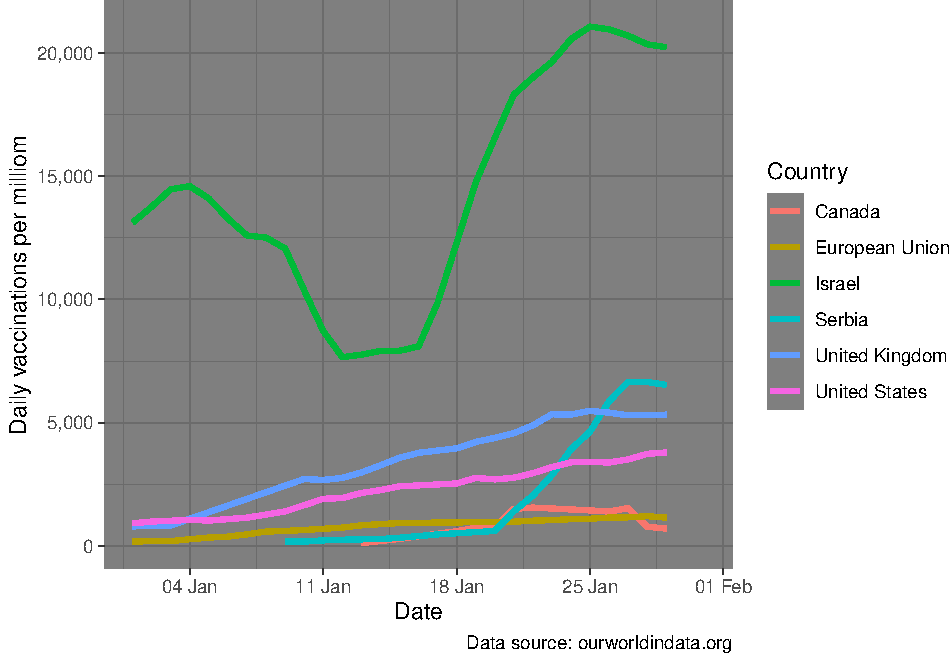
\includegraphics{researchNote_files/figure-latex/unnamed-chunk-5-1.pdf}
\caption{Cumulative vaccine doses of time}
\end{figure}

\hypertarget{discussion}{%
\section{Discussion}\label{discussion}}

\begin{itemize}
\tightlist
\item
  Don't book your summer holidays just yet.
\end{itemize}

\hypertarget{references}{%
\section*{References}\label{references}}
\addcontentsline{toc}{section}{References}

\hypertarget{refs}{}
\leavevmode\hypertarget{ref-pm2021}{}%
1. Press conference - australian parliament house. Published online
January 2021.
\url{https://www.pm.gov.au/media/press-conference-australian-parliament-house-12}

\bibliographystyle{unsrt}
\bibliography{references.bib}


\end{document}
